\chapter{Wykład IX.}

\section{Grupy wolne}

Grupa generowana przez zbiór $\{g_1,\ldots,g_{n} \} $ to grupa, które elementami są iloczyny elementów postaci $g_{i}$ oraz $g_{i}^{-1}$. Chcemy zbudować grupę generowaną przez atrakcyjny zbiór $X = \{x_{i}: i \in I\} $, tak żeby nie zachodziły żadne relacje (równości) oprócz koniecznych w oczywisty sposób  np. $x_{i}x_{i}^{-1}, x_{i}^{-1}x_{j}x_{j}^{-1}x_{i} = e, \ldots$

Mówimy ,,wolna'', myślimy ,,wolna od relacji''.

\begin{definition}
	Mamy:
	\begin{itemize}
		\item Alfabet: $X = \{x_{i}: i \in I\} $.
		\item Słowa nad $X$ : skończone ciągi symboli $x_{i}$ oraz $x_{i}^{-1}$.
		\item Słowo skracalne: to słowo, w którym występują sąsiednie symbole $x_{i}^{\varepsilon }, x_{i}^{-\varepsilon }$, dla pewnych $i\in I$ oraz $\varepsilon \in \{-1,1\} $.
		\item Słowo nieskracalne to słowo, które nie jest skracalne.
		\item $L_{x}$ : zbiór słów na alfabecie $X$.
		\item Relacja równoważności na $L_{x}$ :
			\[
			w\sim v \iff v \text{ powstaje z } w \text{ przez skończoną liczbę wstawień lub skróceń słów postaci } x_{i}^{\varepsilon }, x_{i}^{-\varepsilon } 
			.\] 
		\item $\mathbb{F}_{x} := \mfaktor{L_{x}}{\sim  } $: zamiast $\left[ a \right] _{\sim}$ będziemy pisać $\left[ a \right] $.
	\end{itemize}
\end{definition} 

\begin{theorem}
	Dla $\left[ u \right] , \left[ v \right] \in \mathbb{F}_{x}$ definiujemy
	\[
	\left[ u \right] \cdot \left[ v \right] := \left[ uv \right] 
	.\] 

	Definicja ta nie zależy od wyboru reprezentantów i $\left( \mathbb{F}_{x}, \cdot \right) $ jest grupą z elementem neutralnym $\left[ \emptyset  \right] $.
\end{theorem} 
\begin{proof}
	TODO
\end{proof} 
\begin{theorem}
	W każdej klasie $\left[ u \right] $ istnieje dokładnie jedno słowo nieskracalne.
\end{theorem} 
\begin{proof}
	TODO
\end{proof} 
\begin{definition}
	Dla $u \in L_{x}$, przez $\varsigma \left( u \right)$ oznaczamy jedyne słowo nieskracalne $\sim  $ z $u$
\end{definition} 
\begin{remark}
	Jest to dokładnie funkcja z dowodu twierdzenia 2
\end{remark} 
\begin{corollary}

	Funkcja
	\begin{figure}[H] % [h!] to sugestia, by umieścić "tutaj"
	        \centering
		\adjustbox{scale = 1.0}{
		\begin{tikzpicture}[node distance = 0.4cm and 0.7cm]
	  % Tell it where the nodes are
	  \node (A) {$ X $};
	  \node (C) [right=of A] {$ \mathbb{F} _{X} $};
	  \node (B) [below=of A] {$xi  $};
	  \node (D) at (B -| C) {$\left[ xi \right]   $};
	  % Składnia (B -| C) oznacza: weź współrzędną Y z punktu B i współrzędną X z punktu C
	  % Tell it what arrows to draw
	  \draw[draw=none] (A)-- node[midway] {\small $\rotatein$} (B);
	  \draw[|->] (B)--(D);
	  \draw[-stealth] (A)--(C);
	  \draw[draw=none] (C)-- node [midway] {\small $\rotatein$} (D);
	\end{tikzpicture}}
	\end{figure}
	
	jest różnowartościowa.
\end{corollary}
\begin{proof}
	TODO
\end{proof} 
\begin{remark}
	Jeśli $\left| X \right| = \left| Y \right| $, to $\mathbb{F}_{x}\cong \mathbb{F}_{Y}$. Dokładniej to jeśli $f:X\to Y$ jest bijekcją, to $\overline{f}: \mathbb{F} _{x}\to \mathbb{F} _{Y}$ zadana przez 
	 \[
		 \overline{f}\left( \left[x_{i_1}^{\varepsilon _{i_1}}\ldots x_{\i_{n} }^{\varepsilon_{\i_{n} }} \right]  \right) := \left[ f\left( x_{i_1} \right)^{\varepsilon_{i_1}}\ldots f\left( x_{\i_{n} } \right)^{\varepsilon_{\i_{n} }} \right] 
	\] 
	jest izomorfizmem.
\end{remark} 
\begin{definition}
	Grupę wolną o (wolnym) zbiorze generatorów X nazywamy dowolną grupę $G \supseteq X$ izomorficzną z $\mathbb{F}_{x}$ przez izomorfizm $\varphi: G \to \mathbb{F}_{x}$, takie że
	\[
	\left(\forall x \in X \right)\left( \varphi \left( x \right) = \left[ x \right]   \right)  
	.\] 
\end{definition} 
\begin{remark}
	$\mathbb{F} _{X}$ jest grupą wolną o zbiorze generowanym $\{\left[ x \right] : x \in X\} $. W wniosku (którego?) $\{\left[ x \right] : x \in X\} $ można utożsamić z $X$ i wtedy $\mathbb{F}_{X}$ staje się grupą wolną o zbiorze generatorów $X$. Istnienie grupy wolnej bez tego utożsamienia $X$ z $\{\left[ x \right] : x \in x\} =: \left[ x \right] $ (niewyraźne notatki)
\centering
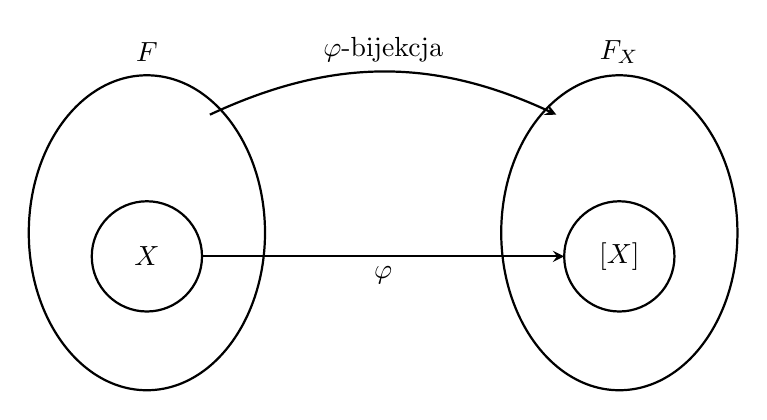
\begin{tikzpicture}[>=stealth, thick]
    % --- LEWA STRONA: Zbiór F ---
    % Główny owal F
    \draw (0,0) ellipse (1.5cm and 2cm);
    \node at (0, 2.3) {$F$};
    
    % Wewnętrzny okrąg (podzbiór)
    \draw (0, -0.3) circle (0.7cm);
    \node (S1) at (0, -0.3) {$X$};

    % --- PRAWA STRONA: Zbiór F_X ---
    \begin{scope}[xshift=6cm]
        % Główny owal F_X
        \draw (0,0) ellipse (1.5cm and 2cm);
        \node at (0, 2.3) {$\mathbb{F}_{X}$};
        
        % Wewnętrzny okrąg (podzbiór)
        \draw (0, -0.3) circle (0.7cm);
        \node (S2) at (0, -0.3) {$\left[ X \right] $};
    \end{scope}

    % --- ODWZOROWANIA (STRZAŁKI) ---
    % Strzałka między głównymi owalami (z góry)
    \draw[->] (0.8, 1.5) to[bend left=25] node[above] {$\varphi$-bijekcja} (5.2, 1.5);

    % Strzałka między wewnętrznymi okręgami
    \draw[->] (0.7, -0.3) -- (5.3, -0.3) node[midway, below] {$\varphi$};
\end{tikzpicture}

$\varphi  $ indukuje grupę na $F$ taką że
\[
\varphi : F \overset{\cong }{\rightarrow} \mathbb{F} _{x}\text{ i } \varphi \left( x \right) \left[ x \right]   
.\] 
\end{remark} 
\begin{context}

	Od teraz przez $\mathbb{F}_{x}$ będziemy rozumieć dowolną grupę wolną o wolnym zbiorze generatorów $X$.
\end{context}

\begin{theorem}
	Dla podzbioru $X$ grupy $G$ następujące warunki są równoważne:
	\begin{enumerate}[label=\arabic*)]
		\item $G$ jest grupą wolną o wolnym zbiorze generatorów $X$ 
		\item $G = \langle x \rangle $ oraz dwa słowa z $L_{x}$ definiują ten sam element grupy $G$ wtedy i tylko wtedy gdy słowa te są równoważne
		\item $G = \langle x \rangle $ oraz słowo z $L_{x}$ definiuje element neutralny w $G$ wtedy i tylko wtedy, gdy słowo jest równoważne ze słowem pustym.
		\item $X$ jest wolnym zbiorem generatorów tzn. $G = \langle X \rangle $ oraz każde niepuste słowo nieskracalne z $L_{x}$ definiuje różny od $e_{G}$ element grupy $G$.
	\end{enumerate}
\end{theorem} 
\begin{proof}
	TODO jako zadanie na liście
\end{proof} 
\section{Przedstawienie grupy wolnej.}

\begin{definition}
	$N_{X}$ jest to zbiór słów nieskracalnych nad $X$.

	Definiujemy $u\cdot v := \varsigma\left( u,v \right) \in N_{X}$, gdzie $u,v \in N_{X}$
	
\end{definition} 
\begin{fact}

$\left( N_{x}, \cdot  \right) $ jest grupą izomorficzną z $\mathbb{F}_{X} $ przez izomorfizm taki że $x \in X \mapsto \left[ x \right] $. 

Zatem $\left( N_{X}, \cdot  \right) $ jest grupą wolną o wolnym zbiorze generatorów $X$.
\end{fact}
\begin{proof}
	TODO
\end{proof} 
\begin{theorem}[Uniwersalnośc grupy wolnej]
	Niech $f:X \to H$ będzie dowolną funkcją z  $X$ w grupę $H$. Wtedy $f$ przedłuża się jednoznacznie do homomorfizmu $\overline{f}: \mathbb{F}_{X} \to H$ 
\[
\begin{tikzcd}[row sep=30pt, column sep=30pt]
X \arrow[dr, "\id"'] \arrow[rr, "f"] & & H \\
& \mathbb{F}_{X} \arrow[ur, "\exists ! \overline{f}", dashed, hook] &
\end{tikzcd}
.\] 
\end{theorem} 
\begin{proof}
	TODO
\end{proof} 
\begin{theorem}
	Załóżmy, że $X\subseteq G$, $G$ jest grupą. Jeśli $\left( G,X \right) $ jest uniwersalna w sensie że
	\[
	\left(\forall f: X \to H \right)\left(\exists ! \overline{f}: G\to H \right)\left( f\subseteq \overline{f} \right)
	,\] 

	gdzie $H$ jest grupą, a $\overline{f}$ homomorfizmem,

	to istnieje
	\[
	\varphi : G \overset{\cong }{\rightarrow} \mathbb{F}_{X} \text{, takie że } \varphi \restriction_{X} = \id_{X}
	.\] 
\end{theorem} 
\begin{proof}
	TODO
\end{proof} 
\begin{corollary}

	Jeśli $X\subseteq G$, gdzie $G$ jest grupą, to następujące warunki są równoważne:
	\begin{enumerate}[label=\arabic*)]
		\item $G$ jest grupą wolną o wolnym zbiorze generatorów $X$.
		\item $\left( G,X \right) $ jest uniwersalna w powyższym sensie
	\end{enumerate}
\end{corollary}
\begin{theorem}
	Jeżeli $\mathbb{F}_{X} \cong \mathbb{F}_{Y}$ to $\left| X \right| = \left| Y \right| $.
\end{theorem} 
\noindent \textbf{Przykłady}

\begin{enumerate}[label=\arabic*)]
	\item $\mathbb{Z} = \langle \underbrace{1}_{\text{wolny generator}} \rangle \cong \mathbb{F}_{1}$
	\item Komu (?) (ping-pong ?)
		\[
		G := \langle \underbrace{\begin{bmatrix} 1 & 2 \\ 0 & 1 \end{bmatrix} , \begin{bmatrix} 1 & 0 \\ 2 & 1 \end{bmatrix} }_{\substack{\text{zbiór wolnych generatorów} \\ \text{grupa wolna w ,,naturze''}}} \rangle \le SL_{2\left( \mathbb{Z}  \right) } \le SL_{2}\left( \mathbb{R}  \right) 
		.\] 
		Zatem $\mathbb{F}_{2} \cong  G \le SL_{2}\left( \mathbb{R}  \right) $
\end{enumerate}
\begin{theorem}
	W grupie $\mathbb{F}_{\{x,y\} }$, grupa generowana przez elementy $x^{n}yz^{n}, n\in \N$ jest przez nie generowana w sposób wolny.
\end{theorem} 
\begin{corollary}

	\[
		\left(\forall n\in \N \right)\left( \mathbb{F}_{n}\longrightarrow \mathbb{F}_{\aleph_0}\longrightarrow \mathbb{F}_{2} \longrightarrow SL_{2}\left( R \right)   \right)  
	.\] 

	Prawe strzałki powyżej oznaczają monomorfizmy - zanurzenia
\end{corollary}

\begin{theorem}[Nielsen-Schreier]
	Podgrupa grupy wolnej jest wolna (ale może mieć więcej generatorów).
\end{theorem} 
\begin{proof}
	POMINIęTy TODO czemu
\end{proof} 
\begin{fact}

	Każda grupa $G$ jest obrazem pewnej grupy wolnej.
\end{fact}
\begin{proof}
	TODO
\end{proof} 
\begin{definition}
	Niech $X$ będzie zbiorem, $A \subseteq \mathbb{F}_{X} (L_{X}?)$. Wtedy
	\[
	\langle X\mid A \rangle := \mfaktor{\mathbb{F}_{X}}{\langle \langle A \rangle  \rangle } 
	.\] 
\end{definition} 
\begin{intuition}
	Grupę $\mathbb{F}_{X}$ wydzielamy przez wszystkie relacje z $A$. (tzn. ,,słowa z $A = e$ ) tak aby była grupą.

	Będzie to największa (uniwersalna) grupa. Będzie to największa (uniwersalna) grupa spełniająca te relacje. Generowana przez warstwy elementów z $X$. 
\end{intuition} 
\noindent \textbf{Notacja} 

Zamiast $\langle \{x_1,\ldots,x_{n}\} \mid \underbrace{\{n_1,\ldots, n_{m}\}}_{\text{słowa lub elementy }\mathbb{F}_{X}} \rangle $
 
piszemy $\langle x_1,\ldots,x_{n} \mid n_1,\ldots,n_{m} \rangle $ 

oraz np. $\langle x,y \mid xy = yx \rangle $ zamiast $\langle x,y \mid xyx^{-1}y^{-1} \rangle $

\begin{fact}

	(Uniwersalność grupy zadanej przez prezentację.) Niech $A \subseteq L_{X}$. Niech $G$ będzie grupą, a $f: X \to G$ funkcją. Załóżmy, że dla każdego słowa $x_{i_1}^{\varepsilon_1} \dots x_{i_m}^{\varepsilon_m} \in A$ zachodzi
\[
f(x_{i_1})^{\varepsilon_1} \dots f(x_{i_m})^{\varepsilon_m} = e_G.
\]
Wtedy istnieje dokładnie jedno przedłużenie $f$ do homomorfizmu $\bar{f}: \langle X \mid A \rangle \to G$.

$x \overset{\text{iloraz}}{\longrightarrow } \mfaktor{\mathbb{F}_{X}}{\langle \langle A \rangle  \rangle } $ dalej notatki nie są wyraźne- nie umiem rozczytać jak diagram wygląda
\end{fact}
\begin{remark}
	Każda grupa ma prezentację, bo jest obrazem grupy wolnej
	\[
	G \cong \mfaktor{\mathbb{F}_{G}}{\langle \langle A \rangle  \rangle } = \langle G \mid A \rangle 
	.\] 
	gdzie $A = \{u \in \mathbb{F}_{G}: u \text{ wyliczone w } G = e_{G}\} $ oraz $\mfaktor{\mathbb{F}_{G}}{\langle \langle A \rangle  \rangle } = \mfaktor{\mathbb{F}_{G}}{A} $

	Tu $A = \ker(\overline{\id_{G}}) $, gdzie $\overline{\id_{G}}: \mathbb{F}_{G} \longrightarrow G$ 

	oraz $\overline{\id_{G}} \supseteq \id_{G}: G \to G$
\end{remark} 

\vspace{1em}

Istotne jest znajdowanie możliwie najprostszych prezentacji. Powyższa taka nie jest (za duże $X$ oraz za duże $A$ )

\noindent \textbf{Przykłady} 
\begin{enumerate}[label=\arabic*)]
	\item $\mathbb{Z}_{n} \mfaktor{\mathbb{Z}}{\langle n \rangle } \cong \mfaktor{\mathbb{F}_{X} = \langle x \rangle \cong \mathbb{Z}}{\langle x \rangle } = \langle x \mid x^{n} \rangle  $ prezentacja grupy $\mathbb{Z}_{n}$
	\item $\mathbb{Z}_{2} \times \mathbb{Z}_{2} \cong \langle x,y \mid x^2,y^2,\left[ x,y \right]  \rangle $ prezentacja $\mathbb{Z}_{2}\times \mathbb{Z}_{2}$
\end{enumerate}
\begin{proof}
	TODO
\end{proof} 
\subsection*{Przepis na prezentację.}

Aby pokazać, że skończenie generowana grupa $G$ ma prezentację $\langle x_1,\ldots,x_{n} \mid \underbrace{u_1,\ldots,u_{n}}_{\text{słowa}} \rangle $ znajdujemy $g_1,g_2,\ldots,g_{n} \in G$ takie że:
\begin{enumerate}[label=\roman*)]
	\item $\langle g_1,\ldots,g_{n}  \rangle = G$ 
	\item $g_1,\ldots,g_{n} $ spełniają relacje $u_1,\ldots,u_{n} $, tzn $a_{i}\left( g_1,\ldots,g_{n}  \right) = e_{G}$
	 \item Sprawdzamy, że $\left| \langle x_1,\ldots,x_{n} \mid u_1,\ldots,u_{n}  \rangle  \right| \le \left| G \right| $
\end{enumerate}
\noindent \textbf{Przykłady}

\begin{enumerate}[label=\arabic*)]
	\item $S_3 \cong \langle x,y \mid x^2, y^3, xyxy \rangle $ 
	\item $D_{n} \cong \langle x,y \mid x^2, y^{n}, xyxy \rangle $
\end{enumerate}
\begin{proof}
	TODO jako zadanie na liście
\end{proof} 
\begin{definition}
	$A$ jest \textbf{wolną grupą abelową} o bazie $X\subseteq A$ gdy $A$ jest grupą abelową zawierającą $X$ oraz
	\[
	\left(\forall f : X \to H \right)\left(\exists ! \overline{f}: A \to H \right)\left( f \subseteq \overline{f} \right), \text{ gdzie } H \text{ grupa abelowa}   
	.\] 
	
	\[
		\begin{tikzcd}[row sep=30pt, column sep=30pt]
			X \arrow[dr, "\id"'] \arrow[rr, "f"] & & H \\
			& A \arrow[ur, "\exists ! \overline{f}", dashed, hook] &
		\end{tikzcd}
	.\] 
\end{definition} 
\begin{remark}
	Ważne:
	\begin{enumerate}[label=\arabic*)]
		\item Dwie wolne grupy abelowe o bazach tej samej mocy są izomorficzne.
		\item Wolna grupa abelowa o bazie mocy $\kappa$ jest izomorficzna z $\mathbb{Z}^{\oplus\kappa}$

			 W szczególności gdy $\kappa < \aleph_0$ to dostajemy $\mathbb{Z}^{\kappa}$ 
		\item Wolna grupa abelowa o bazie mocy $\kappa$ jest izomorficzna z 
			\[
			 \mathbb{F}_{\kappa}^{ab} := \mfaktor{\mathbb{F}_{\kappa}}{\mathbb{F}_{\kappa}^{'}} \cong \langle \{x_{i}: i \in \kappa\} \mid x_{i}x_{j}x_{i}^{-1}x_{j}^{-1},\text{ gdzie } i \neq j \rangle 
			.\] 
		Zatem $\mathbb{F}_{\kappa}^{ab} \cong \mathbb{Z}^{\oplus\kappa}$
	\end{enumerate}
\end{remark} 
